\section{Elektrischer Aufbau}
\label{sec:Elektrischer Aufbau}
Im Zuge der Arbeit wird die Kälteanlage, die zuvor nur manuell betrieben werden konnte, vollständig auf eine SPS umgebaut. Zu berücksichtigen ist dabei die Hardware-Schaltschrank-Architektur des manuellen Betriebes. Für den manuellen Betrieb besaß die Kälteanlage zwei Schaltschränke zur Versorgung der Komponenten mit der Hilfsenergie sowie zur Ansteuerung der Magnetventile und des Vierwegeventils.

Um den Umbau auf eine SPS vollziehen zu können, ist es nötig, das elektrische Konzept für den manuellen Betrieb nachzuvollziehen, um  gleiche Funktionalität und Sicherheit der Kälteanlage im SPS-Betrieb gewährleisten zu können. Es wird versuch,t einen möglichst großen Anteil der Komponenten des manuellen Betriebes  in das neue elektrische Konzept der SPS einzubinden. Nach dem Umbau wird die Kälteanlage ausschließlich über die SPS bedienbar sein. Der manuelle Betrieb über Schalter wird nicht mehr möglich sein. Die möglichen Betriebsmodi der Kälteanlage werden im Abschnitt \ref{sec:Informationstechnischer Aufbau}\textit{informationstechnischen Konzept} erklärt und vorgestellt. 

Das elektrische Konzept umfasst folgende Teilaspekte bzw. -funktionen:

\begin{itemize}
\item Auslesen von Sensoren
\item Stellen von Aktoren 
\item Versorgung der Aktoren/Sensoren mit Hilfsenergie.
\end{itemize}

Das \textit{Auslesen von Sensoren} umfasst das Auslesen von Temperatur, Druck, Massenstrom, Gewichte der Waagen sowie die Ventilöffnungen der Expansionsventile. Das \textit{Stellen von Aktoren} besteht aus der Sollwertvorgabe für die Kompressor- und Verflüssigerventilatordrehzahl, elektrische Heizung sowie das An- und Ausschalten der Ventilatoren vom Verdampfer und Abtauverdampfer. Des Weiteren werden Magnet- und Vierwegeventile geschaltet. 
Die \textit{Versorgung der Aktoren/ Sensoren mit Hilfsenergie} gewährleistet einen sicheren Betrieb der Kälteanlage und die Funktionalität der Komponenten.  
%Der Frequenzumformer des Kompressor wurde manuell über ein Touchpad angesprochen. Über das Touchpad wurde der Sollwert des Saugdruckes vorgegeben.  

Das elektrische Konzept sieht eine zentralisierte elektrische Installation vor. Für die Kälteanlage sind sowohl analoge Ein- und Ausgangssignale (0..10 V DC, 4..20 mA) als auch Digitale Ausgangssignale (0...24 V DC) vorgesehen. Diese Signale werden über maximal 10 m gesendet. Damit ist die Verwendung eines Buskopplersystem nicht erforderlich. Die meisten Signale werden jedoch nur über wenige Meter zu den benachbarten Schaltschränken gesendet. Hierbei ist mit keinen Problemen durch elektromagnetische Störungen zu rechnen. 

Für das Auslesen der Sensoren, die maximal  20 m von dem SPS-Schaltschrank entfernt sind, wird ein Bussystem (MODBUS RTU) eingesetzt. Dieses Bussystem erlaubt es bis zu 32 Sensoren auf einer Entfernung von theoretisch 1000 m anzuschließen. Im Abschnitt \ref{subsec:Modbus} wird das Protokoll \textit{Modbus RTU} und der elektrische Aufbau des Modbuses erklärt. 
 
Die SPS besteht aus dem CPU-Grundmodul \textit{CX9020} sowie Busklemmen der Fa. Beckhoff. Die Busklemmen sind vom Typ E-Bus, die das firmeneigene Protokoll EtherCAT (Ethernet for Control Automation Technology) unterstützen.  Das EtherCAT verfügt neben ihrer Echtzeitfähigkeit(1.000 verteilte I/Os in 30 $\mu s$\citep{Beckhoff2016}) auch über die Fähigkeit zur Einbindung von  Standardethernet Komponenten und flexiblen Typologien. Bei einem E-Bus (ELxxxx)wird das Prozessabbild mittels des EtherCAT
Protokolls, das vom Standard Ethernet Protokoll abgeleitet ist, bis an die jeweilige Busklemme übermittelt. Die Busklemme kann dann ihren Wert lesen bzw. schreiben. Dieses Verfahren erlaubt eine äußerst geringe Zykluszeit. Abbildung \ref{fig:Beckhoffklemmen} zeigt exemplarisch das Grundmodul CX9020 und eine PT100-Temperatur-Busklemme. Der CX9020 verfügt über einen 1-GHz-CPU und läuft mit dem Betriebssystem Windows CE. Es wird auf einer Hutschiene montiert und erkennt angeschlossene Busklemmen automatisch. 

\begin{figure}[htb]
\centering
\subfigure[Ethernet-Steuerungs-CPU CX9020]
{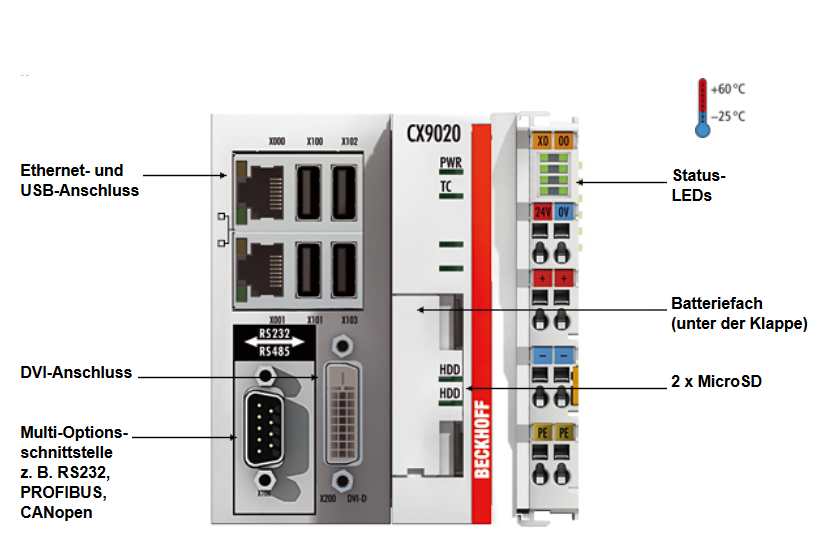
\includegraphics[width=0.52\textwidth]
{Pictures/CX9020.png}}
\subfigure[EL3202: 2-Kanal-Eingangsklemmen für PT100-Temperatursensoren]{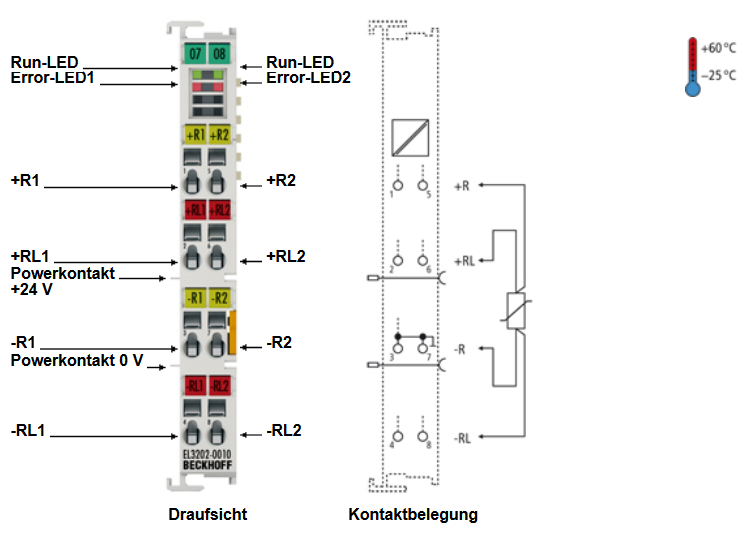
\includegraphics[width=0.42\textwidth]
{Pictures/EL3202.png}}
\caption{SPS-CPU und E-Busklemme der Fa. Beckhoff}
\label{fig:Beckhoffklemmen}
\end{figure}

In Tabelle \ref{tab: Beckhoff-Busklemmen- Übersicht} sind alle verwendeten Klemmen mit Kanalanzahl, Signalart und der eingesetzten Anzahl aufgelistet. 

Der CX9020 verfügt über zwei RJ45 Anschlüsse für LAN-Schnittstellen. Hier können weitere Buskoppler oder ein PC angeschlossen werden. Buskoppler kommunizieren über EtherCAT  und der PC über TCP/IP mit dem Gerät. Eine der zwei Schnittstellen dient zur Kommunikation mit dem Host-PC. Vier USB-Schnittstellen dienen für einen Anschluss von beispielsweise einer Maus, Tastatur  oder eines Speichermediums. 

\begin{table}[htb]
\centering
\caption{Busklemmen-Übersicht}\vspace{6pt}
\begin{tabular}{p{2cm}p{3.6cm}p{1.4cm}p{2.8cm}p{3.2cm}ccccc}
\hline 
\rule[-1ex]{0pt}{2.5ex} \textbf{Klemmennummer} & \textbf{Typ} & \textbf{Anzahl Kanäle} & \textbf{Signal} & \textbf{Eingesetze Anzahl} \\ 
\hline 
\hline 
\rule[-1ex]{0pt}{2.5ex} EL 4024 & Analog Ausgang & 4 & 4..20 mA & 1 \\ 
\hline 
\rule[-1ex]{0pt}{2.5ex} EL 4008 & Analog Ausgang & 8 & 0..10 V DC & 1 \\ 
\hline 
\rule[-1ex]{0pt}{2.5ex} EL 3202 & Analog Eingang & 2 & Temperatur (°C) & 6 \\ 
\hline 
\rule[-1ex]{0pt}{2.5ex} EL 3054 & Analog Eingang & 4 & 4..20 mA & 1 \\ 
\hline 
\rule[-1ex]{0pt}{2.5ex} EL 2809 & Digital Ausgang & 16 & 24 V DC  & 1 \\ 
\hline 
\rule[-1ex]{0pt}{2.5ex} EL 6021 & Serielle Schnittstelle & 1 &  RS422/RS485 & 1 \\ 
\hline 
\rule[-1ex]{0pt}{2.5ex} EL 9410 & E-Bus Auffrischung & 0 & - & 1 \\ 
\hline 
\rule[-1ex]{0pt}{2.5ex} EL 6002 & Serielle Schnittstellen & 2 & RS232 & 3 \\ 
\hline 
\rule[-1ex]{0pt}{2.5ex} EL 9011 & Endklemme & 0 & - & 1 \\ 
\hline 
\hline 
\end{tabular} 
\label{tab:Klemmenübersicht}
\end{table}



Der CX9020 wird über einen Trafo von der Fa. Siemens mit 24 V DC versorgt. Über die Kanäle 24 V und 0 V wird der Buskoppler EK 1200 mit Spannung gespeist. Der EK 1200 kommuniziert per E-Bus mit den angeschlossenen Klemmen und versorgt diese über die Powerkontakte mit Spannung.  Der Buskoppler ist in den den CX9020 integriert. Die EK 1200 stellt eine Stromversorgung von 1860 mA zur Verfügung.  Jede Klemme hat einen Stromverbrauch im Bereich von 50-190 mA. Eine Unterschreitung der 0 mA Grenze ist möglich, kann laut Hersteller jedoch zu Kommunikationsproblemen führen und ist zu vermeiden. Deshalb wird eine E-Bus-Auffrischungsklemme EL 9410 zur Einspeisung weiterer 1860 mA in den E-Bus integriert. 

Jede Klemme verfügt je nach Ausführung über verschiedene Diagnose-LEDs, die Auskunft über korrekten Anschluss, Betriebsstatus oder eventuelle Fehler geben. Die Kommunikation zu den Busklemmen erfolgt über die Kontakte an der Seite (E-Bus). Die Ausführungen der Busklemmen sind sehr vielfältig. Sie unterscheiden sich in der Kanalanzahl, Genauigkeit, Auflösung etc. Abbildung \ref{fig:Beckhoffklemmen} zeigt den CX9020 und eine EL 3202 für zwei PT100-Temperaturelemente. 

Der Beckhoff-Schaltschrank wird über eine separate Spannungsquelle, getrennt von anderen elektrischen Komponenten,  versorgt. Dies erlaubt einen Betrieb der SPS, z. B. fürs Programmieren oder Testen, unabhängig von den anderen Schaltschränken. 

Folgende Komponenten der Kälteanlage werden elektrisch an die SPS angeschlossen: 
\begin{itemize}
\item	Kompressor-Frequenzregelung geregelt mit einem analogem Ausgangssignal 4..20 mA
\item	Verflüssigungsregelung geregelt mit einem analogem Ausgangssignal  0..20 mA
\item	Elektrische Heizungselemente gesteuert mit einem analogem Ausgangssignal mit 0..10 V
\item	Schaltschütze mit digitalem Ausgangssignal 0..24 V DC für Magnetventile, 4-Wegeventil, Spannungsfreigabe für Verdampfer-Ventilatoren
\item 	Modbus RTU über COM-Schnittstelle und RS485-Busklemme
\item 	Waagen-Auslesung über RS232-Schnittstelle
\item 	PT100- Temperaturelemente 
\end{itemize}

Für die genaue elektrische Installation wird an dieser Stelle an die Handbücher der jeweiligen Komponenten verwiesen. Elektrische Arbeiten über 50 V wurden von der elektrischen Werkstatt des Instituts durchgeführt. \citep{MicroNovaAG2011}

\begin{figure}[htb]
\centering		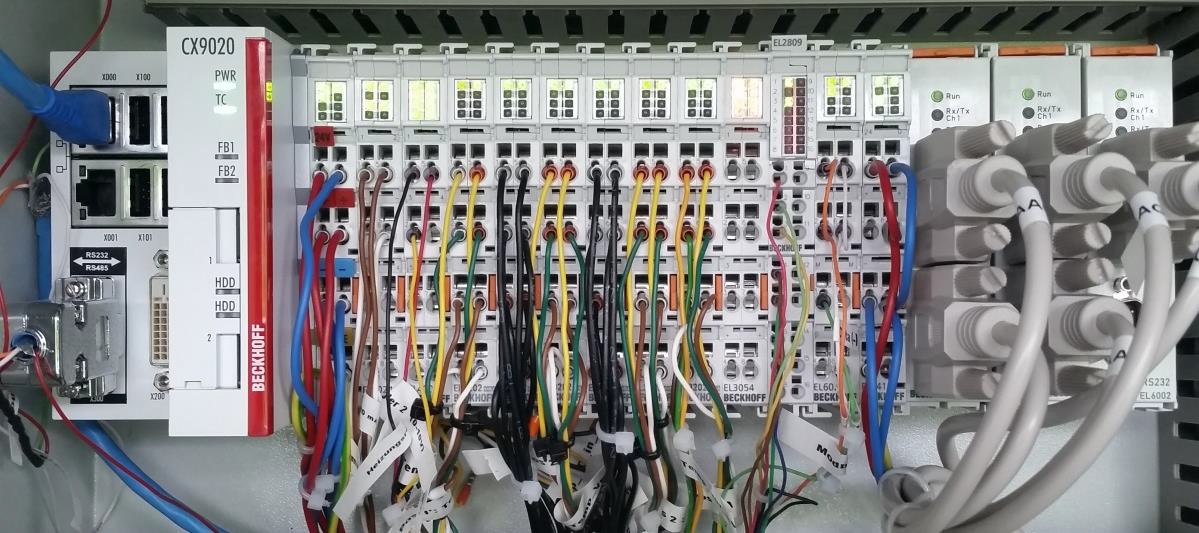
\includegraphics[width=0.90\textwidth]{Pictures/Versuchsaufbau/SPS_BILD.png}
\caption{Verkabelung von CX 9020 und Busklemmen}
\label{fig:}
\end{figure}

\newpage
\subsection{RS232-Kommunikation zwischen SPS und KERN-Waage}
\label{subsec:RS232-Verbindung}


\begin{figure}[htb]
\centering
\subfigure[Waage mit separatem Display vom Typ \textit{PCD 10K0.1} der Fa. \textsc{Kern und Sohn Gmbh} \citep{KERN2006}]
{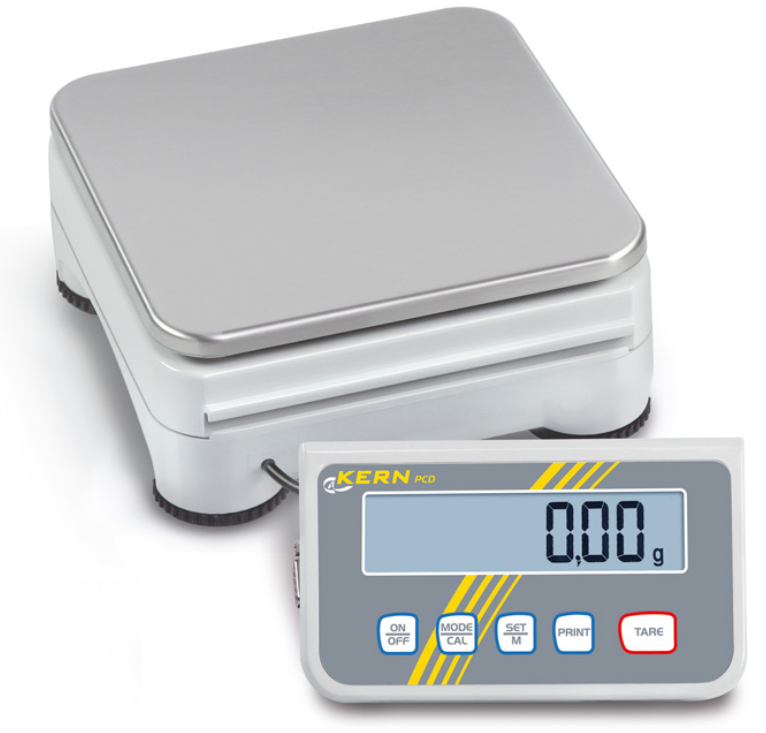
\includegraphics[width=0.4\textwidth]
{Pictures/Waage.png}}
\hspace{2cm}
\subfigure[RS232-Spannungspotentiale von einem nominellen Sender und der EL 6002-Busklemme \citep{Beckhoff2015}]{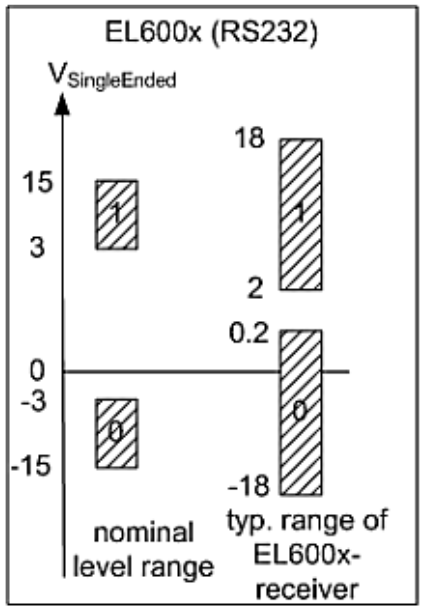
\includegraphics[width=0.3\textwidth]
{Pictures/RS232_spannungspotential.png}}
\caption{Waage mit Spannungspotentiale für eine RS232-Kommunikation}
\label{fig:Waage}
\end{figure}


Das Wägesystem verfügt zurzeit über 5 Waagen, die kontinuierlich von der SPS ausgelesen werden sollen. Jede Waage besteht aus zwei miteinander verbunden Teilen: die Wägeeinheit und das Display mit der RS232-Schnittstelle, vgl. Abbild \ref{fig:Waage}. Das Datenverbindungskabel zwischen Waage und Display wurde verlängert, sodass sich die Displays in der Nähe des SPS-Schaltkrankes befinden. Der Hersteller empfiehlt die Länge von 2 m für die RS232-Verbindung nicht zu überschreiten.  
Über die Datenschnittstelle kann die Waage Befehle empfangen und Messdaten bzw. Fehlermeldungen senden. 

Eine RS232-Kommunikation arbeitet \textit{bitseriell} und diesem Fall mit einem 8-bit ASCII-Code. RS232 ist eine Spannungsschnittstelle. Binäre Zustände werden durch unterschiedliche Spannungspegel realisiert und versendet. Der Spannungspegel für eine RS232-Kommunikation ist in Abbild \ref{fig:Waage}(b) dargestellt. \citep{Schleicher2005}

Hierfür wird ein serielles D-Sub-Kabel benutzt, das an einem Ende einen männlichen D-Sub-Stecker für die EL 6002-Busklemme hat und einen weiblichen D-Sub-Stecker für die Waagen-Schnittstelle. Abbildung \ref{fig:RS232} zeigt die Verkabelung für die RS232-Kommunikation. 

Die Waagen sind in der Klimakammer aufgestellt und ihre Sendeeigenschaften  werden in den Einstellungen auf \textit{AU PC} gestellt. Die Waagen senden dadurch kontinuierlich ihre aktuellen Messdaten an die Klemme, ohne Aufforderung der SPS. Auch wenn die Werte instabil sind, werden sie gesendet. Die Auslesung der gesendet Daten bzw. des Prozessbildes erfolgt dann über Funktionsbausteine und Programme auf der SPS, siehe Abschnitt \ref{sec:Informationstechnischer Aufbau}.

\begin{figure}[htb]
\centering		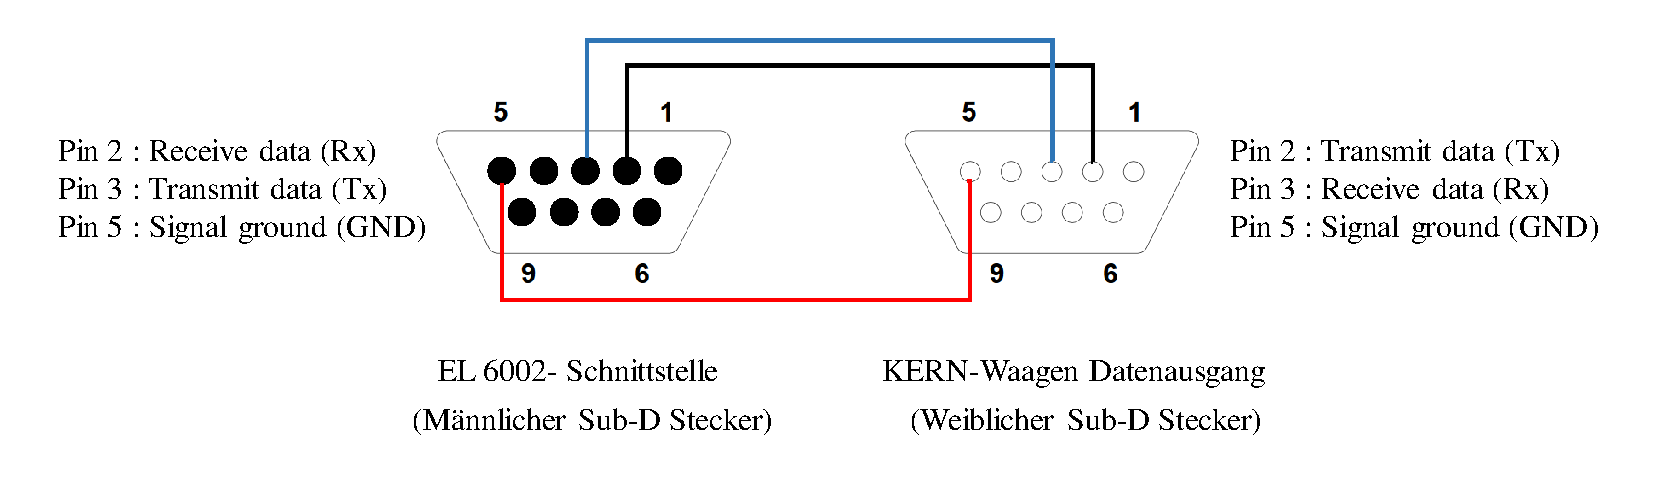
\includegraphics[width=1.05\textwidth]{Pictures/RS232_Verkabelung.pdf}
\caption{Verkabelung für die RS232-Kommunikation zwischen der Busklemme EL 6002 und einer Waage }
\label{fig:RS232}
\end{figure}

\subsection{RS485-Kommunikation zwischen SPS und Sensoren über MODBUS RTU}
\label{subsec:Modbus}

Ein Auslesen von Sensoren kann über analoge Ausgangssignale, z. B. 4-20 mA oder älter 0-20 mA, geschehen oder über Bussysteme. Beide Varianten sind in der Praxis weit verbreitet. Welche Variante zum Einsatz kommt, ist vor allem von der Menge der eingesetzten Sensoren und der Entfernung zwischen ihnen abhängig.
Feldbusse sind nach der Norm IEC 61158 \footnote{\textit{Digital data communication for measurement and control - Fieldbus for use in industrial control systems}} weltweit standardisiert. 

Die Verwendung von Feldbussen hat sowohl Vor- und Nachteile. Die Vorteile sind der geringe Verkabelungsaufwand und die Möglichkeit der Eigendiagnose durch das System selbst. Ein Feldbus-System bietet eine hohe Flexibilität gegenüber Erweiterungen oder Änderung des Netzwerkes. Eine Festlegung auf Messbereiche der Sensoren ist nicht notwendig. Ein weiterer Vorteil ist die Möglichkeit der Abfrage unterschiedlicher Messwerte, wie zum Beispiel Temperatur und Druck, von einem Sensor. Die hohe Zuverlässigkeit und hohe Kompatibilität von verschiedenen Sensortypen ist ein weiterer großer Vorteil.

Die Nachteile eines Feldbusses sind die komplexere Netzwerkstrukturen und -abläufe. Für eine erfolgreiche Implementierung eines Feldbus-Systems wird ein höher qualifiziertes Personal benötigt. Des Weiteren erfordert eine Abfrage der Sensoren meist eine größere Reaktionszeit. Sensoren mit  entsprechender Feldbustechnik sind häufig teurer als Sensoren, die mit analoger Datenübertragung ausgestattet sind. Eine Beschädigung des Kabels kann in manchen Fällen zum Ausfall des kompletten Feldbusses und dessen Sensoren führen. Redundante Netzwerke sind folglich wünschenswert, jedoch nicht immer umsetzbar. 

\begin{figure}[htb]
 \centering		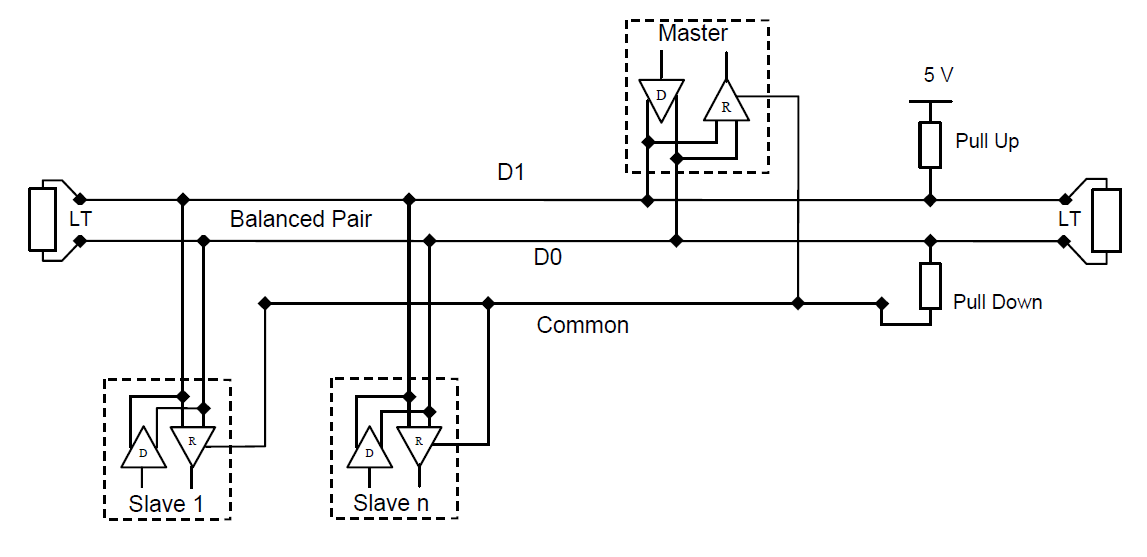
\includegraphics[width=0.94\textwidth]{Pictures/TopologieModbus.png}
 \caption{Zwei-Kabel-Topologie eines MODBUS RTU- Feldbusses \citep{MODBUS.ORG2002}  }
 \label{fig:ZweiKabelModbus}
 \end{figure} 

Feldbusse können mit verschiedenen Netzwerk-Topologien ausgeführt werden. Für den Modbus RTU wird nach \citep{MODBUS.ORG2002} eine Serienschaltung der Hardware-Komponenten (engl. \textit{Daisy Chain}) empfohlen. Die Komponenten sind in dieser Topologie in einer Kette verbunden. Das Signal wird immer an alle Komponenten gesendet und empfangen. Ein Netzwerk besteht zu jeder Zeit aus einem Master und multiplen Slaves. Zunächst schickt der Master einen Befehl an einen Slave. Der Slave setzt den Befehl um und schickt dem Master seine Antwort. Der informationstechnische Aufbau des Modbus RTUs wird im Kapitel \ref{sec:Informationstechnischer Aufbau} beschrieben. 



Ein Modbus RTU kann über ein Vier- oder Zwei-Kabel-Topologie verfügen. Ein Vier-Kabel-Topologie verfügt über zwei paarweise Kabel, über die entweder gesendet oder empfangen wird. Die Befehle über die Sendekabel werden nur vom Master empfangen. Die Befehle über das Empfängerkabel werden hingegen nur von den Slaves empfangen. Beide Kabeltypen sind \textit{monodirektional}.
 
Wird eine Zwei-Kabel-Topologie verwendet, so wird von einer \textit{bi-direktionalen} Verkabelung gesprochen. Die Kabel tragen nach der \textit{EIA/TIA-485 Standard} die Namen $D0$ und $D1$ und werden auch positive und negative \textit{Polarität} genannt. Die Sende- als auch Empfangsbefehle werden von dem Master und allen Slaves empfangen. In beiden Topologiefällen können bis zu 32 Slaves angeschlossen werden und bis auf eine Entfernung von größer 1000 m betrieben werden. 
 
Zusätzlich zu den vier bzw. zwei Kabeln wird ein weiteres Kabel, das \textit{Common}, benötigt. Es stellt ein gleiches Spannungsniveau für alle Slaves sicher. Elektromagnetische Störungen beeinflussen die Datenleitungen ($D0$ und $D1$) und das $Common$-Kabel im gleichen Maße. Die Potentialdifferenz von D1 und D0 zu Common ist folglich konstant. Serielle Bits (0 oder 1) werden mittels Potentialdifferenzen zwischen $D0$ und $D1$ gesendet. Im Falle einer Störung werden diese Bits immer noch vom jeweiligen Receiver erkannt. Somit ist diese Verkabelungsart sehr unanfällig gegenüber elektromagnetischer Störsignale. 


Abbildung \ref{fig:ZweiKabelModbus} zeigt eine typische Zwei-Kabel-Topologie mit Abschlusswiderständen (engl. \textit{Line-Termination}(LT)), einem \textit{Pull-up}- und \textit{Pull-Down}-Widerstand.  Abschlusswiderstände (meist 150 $\omega$, 0.5 W) werden an den zwei Enden der Linientopologie vorgesehen und dienen zur Reduzierung von Signalreflexionen am Ende der Leitungen. Diese können zu Fehlern in der Kommunikation führen. 
Es wird ein \textit{Pull-Up} und ein \textit{Pull-Down} mittels Widerstand zwischen 450 und 650 Ohm durchgeführt. Ein \textit{Pull-Up} zieht die $D1$-Datenleitung auf ein Ruhepotential von 5 V und ein \textit{Pull-Down} die $D0$-Datenleitung auf das Ruhepotential des \textit{Common}-Leiters (meist 0 V).

Die Keller-Drucktransmitter müssen zusätzlich mit Spannung versorgt werden. Die Spannung von 24 V DC wird über eine externe Spannungsquelle gewährleistet und wird in einem Kabelpaar mit 0 V und +24 V zu jedem Drucksensor geführt. Für den Modbus wurden zwei Kontenpunkte am Prüfstand installiert. Von den Kontenpunkten gehen Stichleitungen mit Datenkabeln und bei den Drucktransmittern auch die Spannungsversorgung zu den Slaves ab. Ein Knotenpunkt ist außerhalb der Klimakammer an dem Verflüssigungssatz. Im Abbild \ref{fig:ModbusVerkabelung} sind die Knotenpunkte mit \textit{Kälteanlage} und \textit{Klimakammer} gekennzeichnet. Die Empfehlungen für die Länge der Stichleitung hängt vom Hersteller ab. An diesem Versuchsaufbau sind die Stichleitungen nicht länger als 6 m. 

\begin{figure}[htb]
\centering	
	\includegraphics[page= 2, width=0.8\textwidth]{Pictures/ModbusVerkabelung.png}
\caption{Zwei Modbus-Feldbusse mit angeschlossenen Sensoren, Busklemmen und Spannungsspeisung}
\label{fig:ModbusVerkabelung}
\end{figure}
 
 
  Aufgrund der Inkompatibilität von zwei Slavetypen, \textsc{Keller}- Drucktransmitter und \textsc{CAREL}-Expansionsventilen, wurde ein weiterer Modbus aufgebaut. Genauer wird das Problem in Abschnitt \ref{subsec:Modbus RTU} erklärt. Die Lösung des Problems sind zwei voneinander unabhängige Modbus-Systeme. Ein Modbus wird über die COM-Schnittstelle des CX9020 betrieben und der zweite Modbus über die Klemme EL 6021. Abbildung \ref{fig:ModbusVerkabelung} zeigt die zwei Modbus-Systeme. Der erste Modbus verbindet alle 8 Drucktransmitter und den Massenstromsensor. Der zweite Modbus liest die zwei Expansionsventile aus. Beide Modbus-System sind erweiterbar. 

